\documentclass{article}

\usepackage[letterpaper, portrait, margin=1.5in]{geometry}

\usepackage{fancyhdr}
\usepackage{ragged2e}
\usepackage{graphicx}
\usepackage{caption}
\usepackage{amsmath}
\usepackage{rotating}

\usepackage{listings}
\usepackage{color}

\definecolor{dkgreen}{rgb}{0,0.6,0}
\definecolor{gray}{rgb}{0.5,0.5,0.5}
\definecolor{mauve}{rgb}{0.58,0,0.82}

\lstset{frame=tb,
  language=Java,
  aboveskip=3mm,
  belowskip=3mm,
  showstringspaces=false,
  columns=flexible,
  basicstyle={\small\ttfamily},
  numbers=none,
  numberstyle=\tiny\color{gray},
  keywordstyle=\color{blue},
  commentstyle=\color{dkgreen},
  stringstyle=\color{mauve},
  breaklines=true,
  breakatwhitespace=true,
  tabsize=4
}

\setcounter{secnumdepth}{1}

\usepackage{chngcntr}
\counterwithin{figure}{section}

\renewcommand*{\thepage}{C\arabic{page}}

\pagestyle{fancy}
\lhead{ACME Robotics}
\chead{\#8367}
\rhead{\ifcontents Contents \else Week \thesection \fi}

\newif\ifcontents
\contentstrue

\makeatletter
\renewcommand{\@seccntformat}[1]{}
\makeatother
\begin{document}
\subsection{Finish the console version of the PreScouter}
%! Finish how the PreScouter will be used in the console.
This week, Emma finished the console version of the PreScouter. After calling each request class in Main and making sure that they were all working, Emma set about writing the code that would allow the user to make specific requests with ease. She decided to use a series of if else statements to accomplish this. First, the console asks the user what specific request they would like to make. There are only five requests a user can make because that is the only data that they need from the API. After making a request, Emma uses an if else function to prompt the user for the rest of the information needed in order to complete the URL to send to the API. Then, with the information from the user, Emma pieces together the URL and makes the GET request.\\

At the end of the sendGet() method, Emma used another if else function to print out the data. She decided to use another if else statement because it was easy to use the request from the beginning of the program in order to call the specific class that parsed the data. After she got that all working, the console version of the PreScouter was complete. \\


\subsection {Design double sampling paths}
%Design paths that sample both sets of minerals for extra points in autonomous

While supporting ARES at one of their qualifiers, Kelly saw that many teams either had no auto, or had an auto that only deployed from the lander. Kelly decided that this would make a auto that could disturb both of the gold minerals would be really good to have. In the scenario where an alliance partner did not leave the lander during auto, the location they started at would not matter, so these paths would only have to be designed for ACME's prefered start location, next to the crater. After experimenting by pushing the robot around, Kelly found that there was not enough room between the parked robot and the sampling field to approach the sampling field from the lander side, so the robot would have to first enter the depot, and then push the gold mineral toward the parked robot. This also happened to be an easier modification to make, because it only required duplicating the depot waypoint where the robot dropped off its marker, and adding a waypoint between them to disturb the gold mineral. Kelly tested the paths and found that they worked!

\begin{figure}
    \centering
    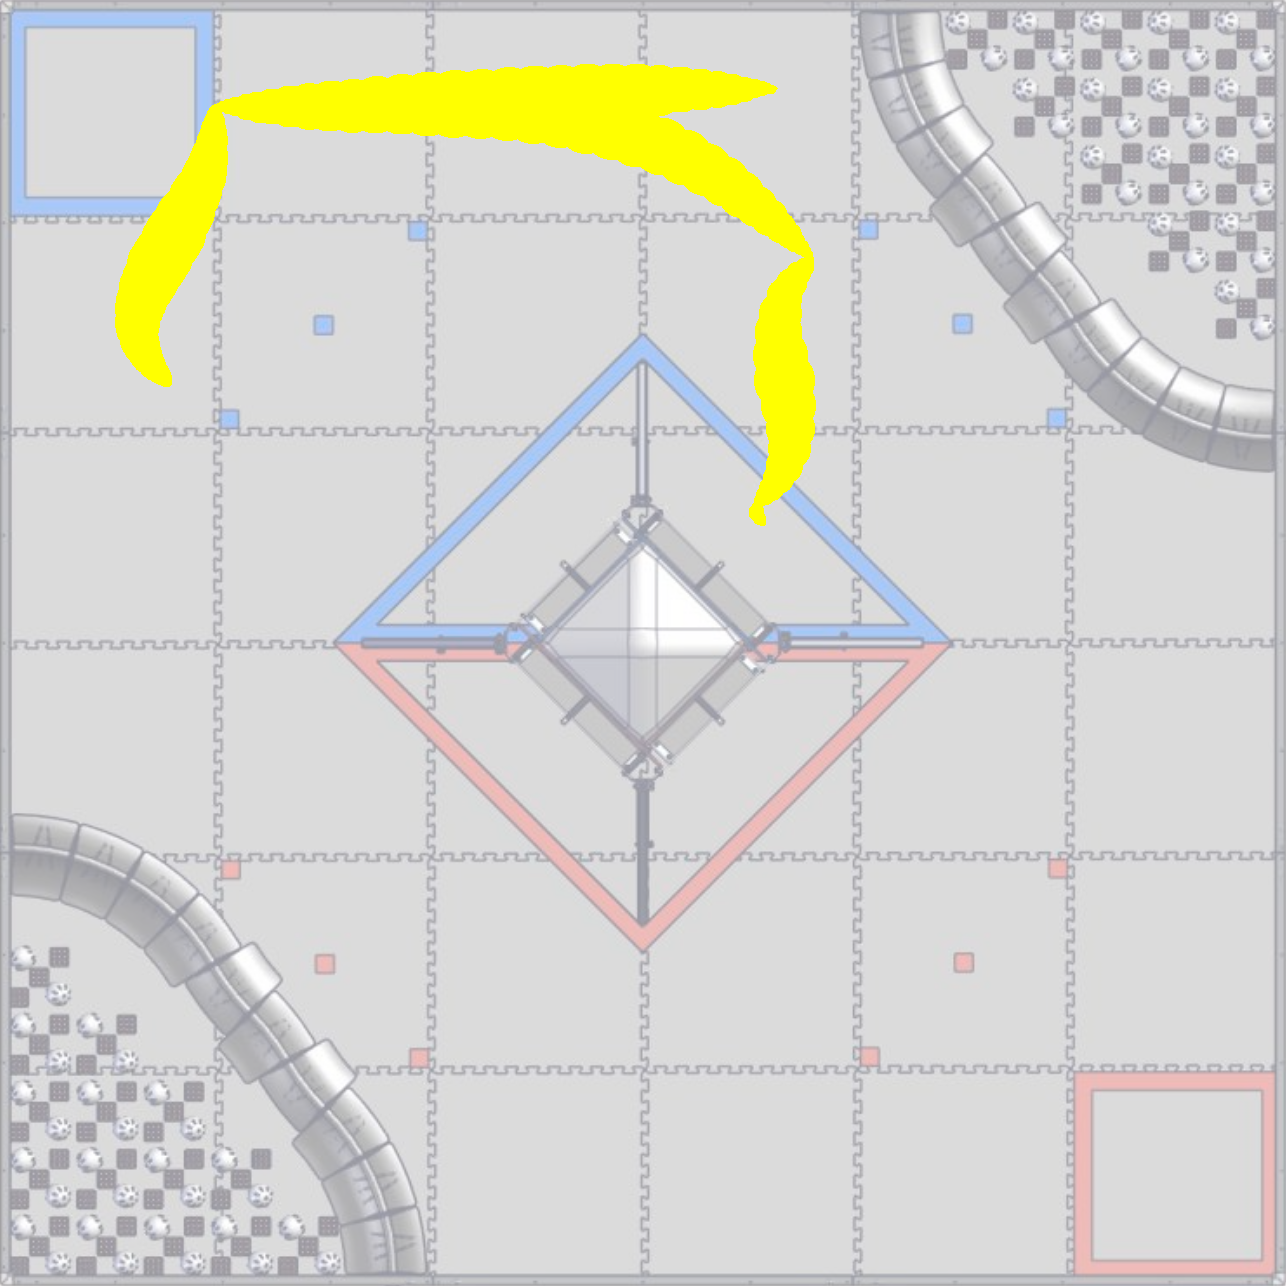
\includegraphics[width=.6\textwidth]{22_01-28/double.png}
    \caption{Double sampling path (line thickness corresponds to robot velocity)}
    \label{fig:double}
\end{figure}

\end{document}